\section{Question 5: Language Modeling}

\subsection{Dataset Description}

Question 5 uses the raw \nolinkurl{wikitext-2-raw-v1} split from WikiText-2 \cite{merity2016wikitext}. The final full-data run used here evaluates 23{,}645 training lines, 2{,}460 validation lines, and 2{,}861 test lines, corresponding to 2{,}051{,}788, 213{,}885, and 241{,}181 tokens after preprocessing. This is therefore a substantially larger and more realistic language-modeling setup than the earlier capped comparison.

WikiText-2 remains appropriate because it contains longer-form Wikipedia prose rather than isolated short sentences. That makes it useful for testing both local collocations and longer-range continuation behavior. The final aligned Q5 section below focuses on the strongest finished full-data trainable model in the new output bundle: the word-level LSTM language model.

\subsection{Model and Preprocessing}

The full-data run uses lowercase word-level tokenization, a minimum token-frequency threshold of 2, vocabulary capping at 30{,}000 tokens, and a maximum BPTT sequence length of 35. The model itself is a two-layer LSTM \cite{hochreiter1997lstm} with 400-dimensional embeddings, hidden size 400, dropout 0.3, tied input-output weights, batch size 32, and AdamW optimization with learning rate \(10^{-3}\). Gradient clipping is set to 0.25.

This run also enables a ReduceLROnPlateau scheduler. Validation perplexity is monitored for early stopping, and the learning rate drops by a factor of 0.25 when progress stalls. That scheduler behavior matters for interpretation because the run continues improving steadily for many epochs before flattening.

\subsection{Results}

Table~\ref{tab:q5_overall_results} reports the final full-data LSTM result. The model reaches validation perplexity 162.79 and test perplexity 151.87, with the best validation point reached at epoch 14.

\begin{table}[H]
\centering
\small
\begin{tabular}{lccc}
\toprule
Model & Best Validation Perplexity & Test Perplexity & Best Epoch \\
\midrule
LSTM & 162.79 & 151.87 & 14 \\
\bottomrule
\end{tabular}
\caption{Full-data Q5 LSTM performance on WikiText-2 raw with 23{,}645 training lines, 2{,}460 validation lines, and 2{,}861 test lines.}
\label{tab:q5_overall_results}
\end{table}

Figure~\ref{fig:q5_lstm_training_curve} shows a smooth optimization trajectory. Validation perplexity falls sharply from 289.39 at epoch 1 to 162.79 at epoch 14, after which it plateaus and then worsens slightly. The scheduler reacts to that plateau by lowering the learning rate from 0.001 to 0.00025 at epoch 17, but the best held-out result had already been reached by then.

\begin{figure}[H]
	\centering
	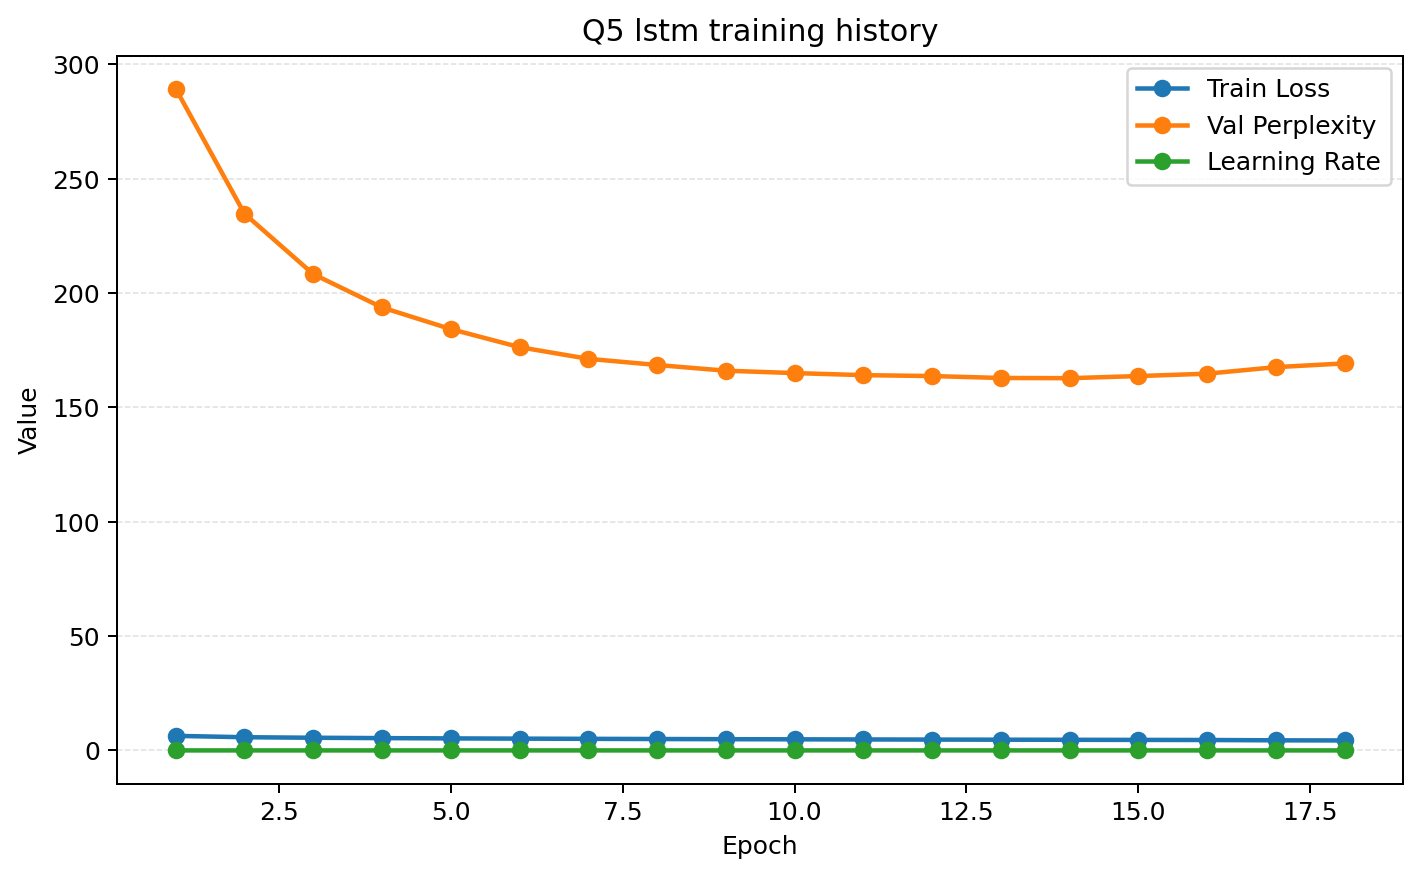
\includegraphics[width=0.82\textwidth]{figures/q5/lstm_training_curve.png}
	\caption{Per-epoch training loss and validation perplexity for the full-data Q5 LSTM run.}
	\label{fig:q5_lstm_training_curve}
\end{figure}

The main result is that the full-data LSTM is no longer a toy baseline. A test perplexity of 151.87 on raw WikiText-2 is still far from state-of-the-art transformer language modeling, but it is strong enough to show that the model has learned reusable sequential structure rather than only memorizing local bigram-like patterns.

\subsection{Generated Text Samples}

The exported generations are consistent with the perplexity curve: the model has learned local syntax and short-range discourse continuation, but its semantic control remains weak. For the prompt ``in the,'' it generates \textit{in the early 1980s , the then use of video numbers are taken 30 million people regarding any more modern state moments .} The start of the sentence is plausible and syntactically recognizable, but later tokens drift into semantically incoherent phrasing.

The other prompts show the same pattern. The seed ``the'' produces a continuation with recognizable function-word structure and topical fragments around books, championships, and teams, but no coherent sentence-level plan. The seed ``he was'' yields a longer continuation with article-noun and clause-like structure, yet the phrase sequence remains semantically unstable. In other words, the model has learned how English Wikipedia-style text tends to sound locally, even though it still struggles to maintain meaning over longer spans.

\subsection{Discussion}

The finished Q5 section now shows that a properly trained full-data LSTM can become a credible language-model baseline on WikiText-2. Its validation curve is smooth, the best checkpoint is easy to identify, and the final held-out perplexity is much better than the earlier smaller-budget recurrent runs.

At the same time, the generated samples show why this is still a baseline rather than a final model: local fluency improves much faster than semantic consistency. The most defensible Q5 claim is therefore that recurrent language modeling benefits strongly from full-data training and scheduling, but that a stronger pretrained causal transformer would still be the natural next comparison if a full-data reference run is added later.